Similar to C2/D2, ratios of \textit{n-subjettiness} variables $\tau_N$~\cite{bib:nsub} can be used to distinguish between different jet topologies. For tagging of top jets the observable
\begin{equation*}
\tau_{32} = \frac{\tau_3}{\tau_2}  
\end{equation*} 
is often used. N-subjettiness $\tau_N$ quantifies the level of agreement between a given \larger jet and a certain number $N$ of subjet axes. The two mainly used subjet axes definitions are $k_\mathrm{t}$-axes, defined by the four-momenta of the $k_\mathrm{t}$-subjets, and the $k_\mathrm{t}$-WTA (Winner Takes All) axes,  corresponding to the four-momentum of the hardest constituent in each $k_\mathrm{t}$-subjet. Throughout this study, the $k_\mathrm{t}$-WTA axes definition is used. The jet is reclustered with an exclusive $k_\mathrm{t}$-algorithm that is executed until the constituents are clustered into $N$ subjets. N-subjettiness is defined as
\begin{equation}
\tau_N = \frac{1}{d_0}\sum_k p_{T,k}\:min(\Delta R_{1,k},\Delta R_{2,k},...,\Delta R_{N,k})^{\beta}\,.
\label{eq:taun}
\end{equation}
The $p_{\mathrm{T}}$ of the constituents $k$ is multiplied by the angular distance to the nearest subjet axis. The relative contributions of the \pt and angular parts can be adjusted through the exponent $\beta$, similar to energy correlation functions. The overall value is normalised with 
\begin{equation*}
d_0=\sum_k p_{T,k}R\,.
\end{equation*}
N-subjettiness is an infrared and collinear-safe variable for values of $\beta \ge 0$.

Small values of $\tau_N$ correspond to a jet with all constituents closely aligned to the given $N$ subjet axes. Hence, the jet is compatible with the assumption to be composed of $N$ or fewer subjets. A high value of $\tau_N$ indicates consistency with more than $N$ subjets, i.e., a sizeable fraction of constituents is located away from the $N$ subjet axes. 
Consequently, top jets are likely to feature a small $\tau_3$ and a high $\tau_2$ value. By contrast, QCD jets with their one-prong structure result in a high $\tau_{3}$ and a small $\tau_{2}$ value. While $\tau_2$ and $\tau_3$ alone provide only small separation, their ratio is a powerful discriminant. A top tagging example with $\tau_{32}$ calculated with clusters in given in Fig.~\ref{fig:nSub_example}. The $\tau_{21}$ ratio can as well be used to tag $W$ or Higgs jets; however, C2 and D2 were found to yield higher background rejections for $W$ tagging~\cite{bib:w_tagging}. 
\begin{figure}
\centering
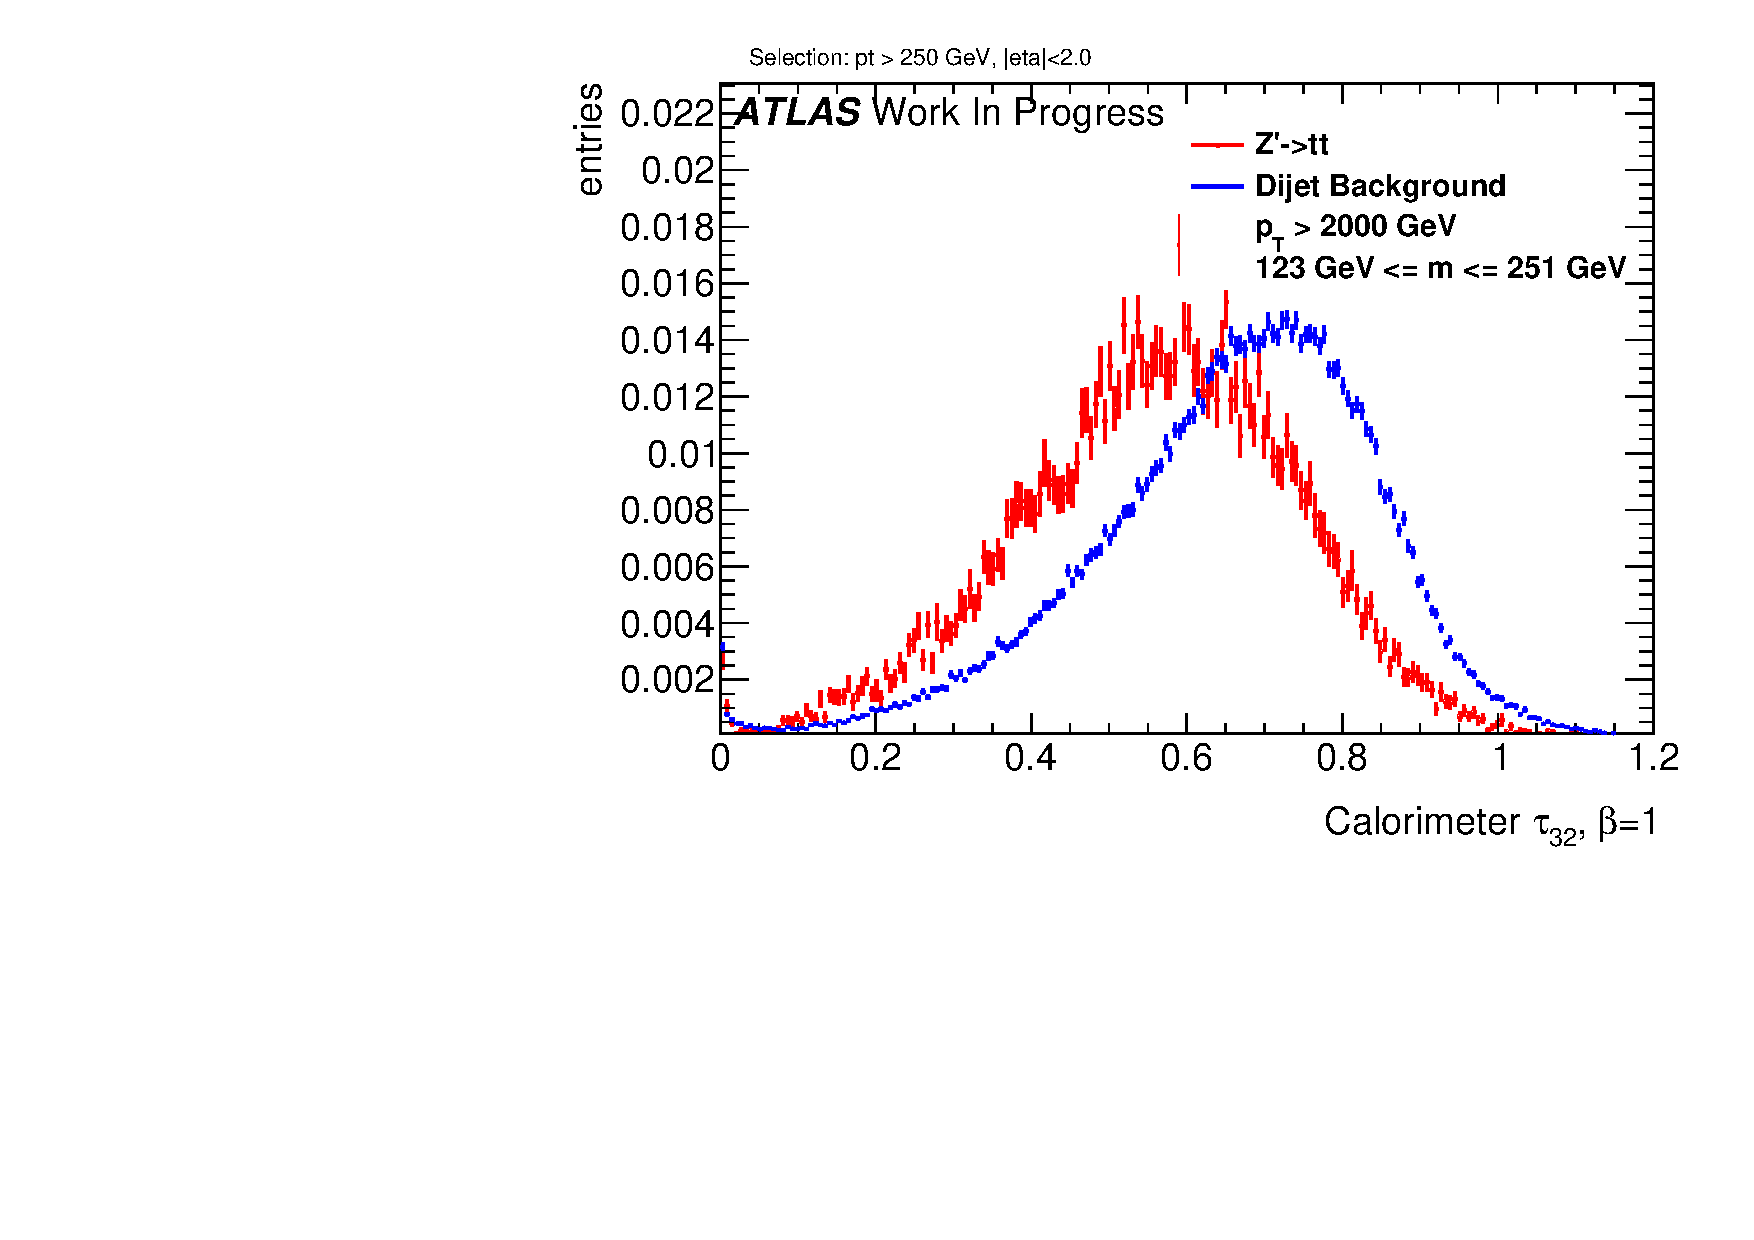
\includegraphics[width=0.6\textwidth]{sascha_input/plots/Top/Beta1/h_recoJet_nSub32_bin6.pdf}
\caption{Representative $\tau_{32}$ distributions for top jets and QCD background jets, calculated from calorimeter clusters. The background tends to higher values.}\label{fig:nSub_example}
\end{figure}

\subsubsection{Jet Substructure Observables from Subjet-Assisted Tracks}
The concept of assisting tracks with the $p_{\mathrm{T}}$ ratio of the whole jet like for \mta has by construction no effect on the studied substructure variables. This can be understood from the definitions of the weighted $p_{\mathrm{T}}$ sums in Eqs.~\eqref{eq:ECF} and~\eqref{eq:taun}. If all tracks are assisted with the same ratio, their three-momenta are scaled by the same factor $c$, which then can be put in front of the sum and cancels as soon as the ratios $\tau_{21}$ and $\tau_{32}$, respectively C2 and D2 are formed:
\begin{equation}
\begin{aligned}
 \tau_N &=& \frac{1}{d_0}\sum_k p_{T,k} \; c \; min(\Delta R_{1,k},\Delta R_{2,k},...,\Delta R_{N,k})^{\beta}\,, \\
 &=& \frac{c}{d_0}\sum_k p_{T,k}\:min(\Delta R_{1,k},\Delta R_{2,k},...,\Delta R_{N,k})^{\beta}\,.
\end{aligned}
\end{equation}
However, assisting tracks using subjets as in Section~\ref{sec:tasalgo} for $\mtas$ is a non-trivial transformation because different scaling factors are used for the tracks, depending on which subjet $c_k$ they are matched to. This results in 
\begin{equation}
\tau_N = \frac{1}{d_0}\sum_k p_{T,k} \; c_k \; min(\Delta R_{1,k},\Delta R_{2,k},...,\Delta R_{N,k})^{\beta}\,.
\end{equation}\label{eq:tas_ta}
The correction works analogously for C2 and D2. In this note, the performance of C2, D2, $\tau_{32}$, and $\tau_21$ will be studied using three inputs:
\begin{itemize}
\item
calorimeter clusters;
\item
subjet-assisted tracks;
\item
tracks which are topologically matched to the \larger jet {\em after} trimming.
\end{itemize}
